\documentclass[12pt]{article}
\usepackage{enumitem}
\usepackage{amssymb}
\usepackage{amsmath}
\usepackage{amsfonts}
\usepackage{mathtools}

\usepackage{clrscode3e}

\usepackage[left=0.5in,right=1in]{geometry}
\renewcommand{\baselinestretch}{1.5}
\newcommand{\sigmastar}{\Sigma^*}

\DeclarePairedDelimiter\floor{\lfloor}{\rfloor}

\begin{document}

\section{Code and Distance}

\subsection{Definition: Code}
A code $C$ of block length $n$ over a finite alphabet $\Sigma$ is any subset of $\Sigma^n$.

$$ C \subseteq \Sigma^n$$

\begin{center}
  "the set of all possible codewords"
\end{center}

e.g. $\Sigma = \{0,1\}$, $n=5$, $C = \{00000, 11111, 00001\}$

\subsection{Definition: Dimension of a Code}
Given a code $C \subseteq \Sigma^n$, $C$ has dimension $k$ defined by:

$$ k = log_{\lvert \Sigma \rvert} \lvert C \rvert $$

\begin{center}
  "n is the size of any codeword"
\end{center}
\begin{center}
  "k is the size of any decoded codeword"
\end{center}

Note: $k \leq n$

e.g. $\Sigma = \{0,1\}$, $n=5$, $C = \{00000, 00001, 00010, 00011, 00100, 00101, 00110, 00111\}$ then, $ k = log_2 (8) = 3$

\subsection{Definition: Rate of a code}
Given a code $C \subseteq \Sigma^n$ with dimension $k$, $C$ has rate $R$ defined by:
$$ R = \frac{k}{n}$$

\begin{center}
  "R is the ratio of non-redundent bits, higher is better, lower means more rendency"
\end{center}


\subsection{Definition: Hamming Distance}
The Hamming Distance between two equal length strings is the number of elementwise differences.

$$d_H = \lvert \{ i \mid x_i \neq y_i \} \rvert$$

e.g. $d_H(bbb, aaa) = 3$

e.g. $d_H(xyz, abc) = 3$

\subsection{Definition: Minimum distance of a code}
Given a code $C \subseteq \Sigma^n$, $C$'s minimum distance $d$ is the smallest distance between any two codewords in $C$.

$$d = min \{d_H(i,j) \mid i,j \in C, i \neq j \}$$

\subsection{Note: [n,k,d]}
Given a code $C$, with dimension $k$, block length $n$ and minimum distance $d$, we call $C$ an $[n,k,d]$ code. These statements hold:

\begin{enumerate}
  \item The maximum number of errors that an [n,k,d] code can correct is $\floor*{\frac{d-1}{2}}.$

  \item The maximum number of errors that an [n,k,d] code can detect is $d-1$
\end{enumerate}
\break

\section{Linear Codes}

\subsection{Field}
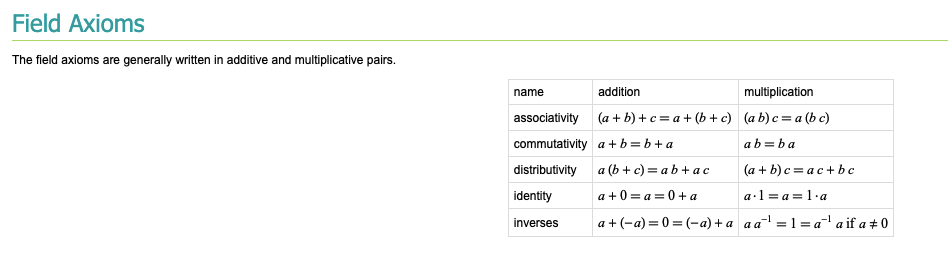
\includegraphics[scale=0.5]{field.png}

\subsection{Finite(Galois) Field}
Is a field that contains a finite number of elements. 

e.g. $GF(2)$ is a finite field with elements $ \{0, 1\}$ addition defined as XOR and standard multiplication.

\subsection{Definition: Linear Code}
We say that $C \subseteq \Sigma^n$ is a linear code if $C$  is a linear subspace of $\Sigma^n$ where $\Sigma$ is a finite field. i.e.:

\begin{enumerate}
  \item $0 \in C$
  \item $\forall a,b \in C, a+b \in C$ 
\end{enumerate}

\break

\section{Error Correction}

Any codeword with enough noise can be any other codeword... we want to be resilient to small noise. 

\subsection{Definition: Encoding Function}
Given a code $C \subseteq \Sigma^n$, a mapping $E: \Sigma^k \rightarrow \Sigma^n$ is called an encoding function.


\subsection{Definition: Decoding Function}
Given a code $C \subseteq \Sigma^n$, a mapping $D: \Sigma^n \rightarrow \Sigma^k$ is called an decoding function.\\ 
Note: $D$ is not injective ... since many codewords may get error corrected to the same decoded codeword 

\subsection{Definition: Error Correction}
Given a code $C \subseteq \Sigma^n$, and an integer $t \in \mathbb{Z}$. $C$ is said to be a $t$ error-correcting code if there exists a decoding function $D$, such that for any $m \in \Sigma^k$ and any noise $\epsilon \in \Sigma^n$ with at most $t$ errors, $D(E(m) + \epsilon) = m$.

\break

\subsection{Example: Repetition Code}

Recall : $GF(2)$ is a finite field with elements $ \{0, 1\}$ addition defined as XOR and standard multiplication.


$C_{3,rep}$ is a 1-error correcting code. Suppose:
$$C_{3,rep} = \{(0,0,0), (1,1,1)\} \subseteq GF(2)^{3}$$
$$E: GF(2) \rightarrow C_{3,rep}$$ 
$$D: GF(2)^{3} \rightarrow GF(2)$$

With functions:
$$ E(x_1) = (x_1, x_1, x_1) $$
$$ D(x_1, x_2, x_3) = (majority(x_1, x_2, x_3))$$ 



e.g. $m = 0, \epsilon = (0,1,0)$, then $D(E(m) + \epsilon) = D(0,1,0) = 0$ 

e.g. $m = 1, \epsilon = (0,1,0)$, then $D(E(m) + \epsilon) = D(1,0,1) = 1$ 


\break

    
\end{document}